
\begin{figure}
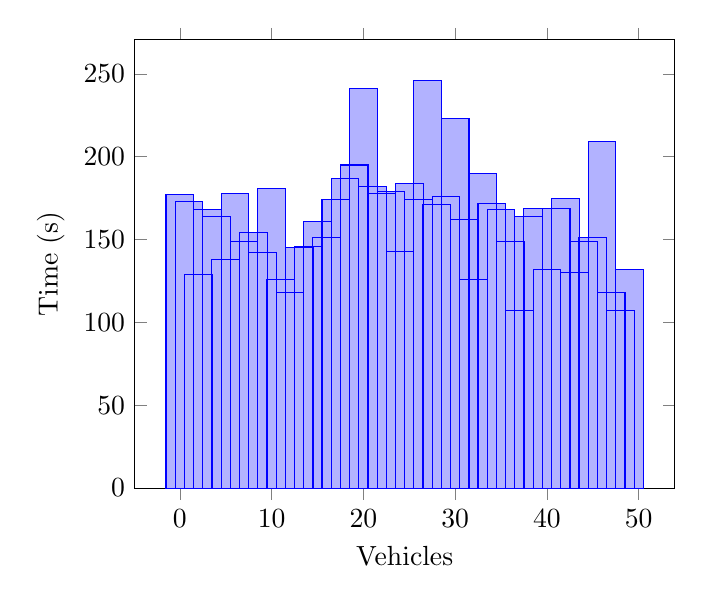
\begin{tikzpicture}
\begin{axis}[
legend style={anchor=west},
xlabel=Vehicles,
ylabel=Time (s),
ymin=0,
ybar,
]
\addplot coordinates {
(0, 177)
(1, 173)
(2, 129)
(3, 168)
(4, 164)
(5, 138)
(6, 178)
(7, 149)
(8, 154)
(9, 142)
(10, 181)
(11, 126)
(12, 118)
(13, 145)
(14, 146)
(15, 161)
(16, 151)
(17, 174)
(18, 187)
(19, 195)
(20, 241)
(21, 182)
(22, 178)
(23, 179)
(24, 143)
(25, 184)
(26, 174)
(27, 246)
(28, 171)
(29, 176)
(30, 223)
(31, 162)
(32, 126)
(33, 190)
(34, 172)
(35, 168)
(36, 149)
(37, 107)
(38, 164)
(39, 169)
(40, 132)
(41, 169)
(42, 175)
(43, 130)
(44, 149)
(45, 151)
(46, 209)
(47, 118)
(48, 107)
(49, 132)
};

\end{axis}
\end{tikzpicture}
\label{tik:0:18_N, 18_N.-60, 17_N, 15_S, 15_S.-30, 13_N, 13_N.-40, 11_N, 8_N, 7_N, 7_N.-60, 5_N, 4_N, 4_N.-60, 1_N}
\caption{0 percent diving with GSC on route $18_N, 18_N.-60, 17_N, 15_S, 15_S.-30, 13_N, 13_N.-40, 11_N, 8_N, 7_N, 7_N.-60, 5_N, 4_N, 4_N.-60, 1_N$}
\end{figure}
